\section{Einleitung und Versuchsziel}
\label{sec:aufgabenstellung}
%In der Aufgabenstellung wird (in eigenen Worten und ganzen Sätzen) formuliert, was das Ziel des 
%Versuches ist.  
%[Beachten Sie die eigentliche Aufgabenstellung in den Versuchsanleitungen sowie die Hinweise zur Auswertung!] 

Im folgenden Versuch werden aus handelsübliche Nelkenblüten die ätherischen Öle extrahiert und charakterisiert. Wesentliche Arbeitsmethoden sind bei diesem Versuch die Wasserdampfdestillation, das Extrahieren, sowie das Rotationsverdampfen. Die ätherischen Öle der Nelken werden massenspektrometrisch per  Gaschromatografie detektiert.\\
Die Hauptkomponenten der ätherischen Öle der Nelke, die in diesem Versuch extrahiert wurden, wird nach Recherchen mit den Verbindungen \textit{Eugenol}, \textit{Eugenolacetat} und \textit{$\beta$-Caryophyllen} beschrieben \cite{Berger.2017,Krammer.2003,ROMPPRedaktion.2002}.


\begin{figure}[h!]
	\begin{minipage}{0.32\textwidth}
			\resizebox{5cm}{!}{
			\chemfig{=[-1]-[1]-[-1]*6(=-=-(-O-[-1]CH3)=-)}}
			\caption{Strukturformel Eugenol}\label{fig:eugenol}
	\end{minipage}\hfill
	\begin{minipage}{0.32\textwidth}
		\resizebox{5cm}{!}{
			\chemfig[angle increment=30]{=[-1]-[1]-[-1]*6(=-=-(-O-[-1]CH3)=(-O-[1](=[-1]O)-[-45]CH3)-)}}
			\caption{Strukturformel Eugenolacetat}\label{fig:eegenol_ac}
	\end{minipage}\hfill
	\begin{minipage}{0.32\textwidth}
			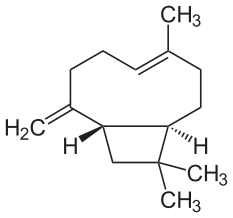
\includegraphics[width=0.8\textwidth]{img/caro}
			\caption{Strukturformeln $\beta$-Carophyllen}\label{fig:caro}
	\end{minipage}\hfill
\end{figure}
\FloatBarrier

\chemfig{	HO-[,0.75]\chemabove{N}{\scriptstyle\oplus}
			(=[1,0.75]\lewis{02,O})
			-[7,0.75]\chemabove{\lewis{157,O}}{\scriptstyle\ominus}}
		
\chemfig{	HO-[,0.75]\chemabove{N}{\scriptstyle\oplus}
	(=[1,0.75]\lewis{02,O})
	-[7,0.75]\chemabove{\lewis{157,O}}{\scriptstyle\ominus}}	
		




